\documentclass[conference]{IEEEtran}
\usepackage[utf8]{inputenc}
\usepackage[T1]{fontenc}
\usepackage[brazil]{babel}
\usepackage{amsmath,amssymb}
\usepackage{booktabs}
\usepackage{graphicx}
\usepackage{cite}
\usepackage{url}
\usepackage{hyperref}
\usepackage{placeins}

\graphicspath{{figures/}}

\begin{document}

\title{Classificação multiclasse de janelas de FBGs para demodulação de sensores LPFG}

\author{
\IEEEauthorblockN{Jakson da Rocha Almeida}
\IEEEauthorblockA{Universidade Federal de Juiz de Fora (UFJF)\\
Juiz de Fora, MG, Brasil}
\and
\IEEEauthorblockN{Felipe Oliveira Barino}
\IEEEauthorblockA{Departamento de Circuitos, UFJF\\
Juiz de Fora, MG, Brasil}
}

\maketitle

\begin{abstract}
Sensores LPFG oferecem alta sensibilidade, mas sua interrogação espectral convencional é cara.
Uma alternativa \emph{modula} o espectro da LPFG com um array de FBGs e estima $\lambda_{res}$ por aprendizado de máquina.
Observamos que as quatro FBGs mais próximas de $\lambda_{res}$ formam sempre uma janela contígua; isso permite reduzir a seleção de canais a dez classes $C_s=\{s,\ldots,s+3\}$.
Avaliamos seis classificadores clássicos em $7300$ amostras reais, com nested CV e hold-out estratificado.
SVM e Random Forest atingem acurácia $0{,}938$ no hold-out; a análise mostra erros predominantemente entre janelas adjacentes e impacto do desbalanceamento de classes.
O resultado apoia uma arquitetura em duas etapas: classificar a janela e, em seguida, estimar $\lambda_{res}$.
\end{abstract}

\begin{IEEEkeywords}
Classificação multiclasse, FBG, LPFG, reconhecimento de padrões, sensores ópticos.
\end{IEEEkeywords}

\section{Introdução}

Redes de período longo em fibra (LPFG) acoplam o modo fundamental a modos de revestimento e atuam como filtros de rejeição de banda, viabilizando sensores de índice de refração, temperatura e outras grandezas~\cite{James1996LPFG}.
Em contraste, as redes de Bragg (FBG) apresentam pico de reflexão estreito e contam com cadeias de interrogação relativamente maduras e comercialmente disponíveis~\cite{Kersey1997FBG}.
Essa assimetria faz com que a leitura direta do vale ressonante de uma LPFG --- tipicamente via analisador óptico de espectro --- permaneça um obstáculo de custo para aplicações em campo e para multiplexação em redes densas de sensores.

Uma linha recente combina um array de FBGs, operando como banco de filtros, com modelos de aprendizado de máquina para recuperar o comprimento de onda ressonante $\lambda_{res}$ da LPFG a partir das potências refletidas~\cite{Barino2020Sensors,Barino2024LAWOFS,Barino2025TIM}.
Em~\cite{Barino2025TIM}, um modelo com autoatenção treinado em dados sintéticos e validado em medidas reais reporta RMSE de $0{,}75$~nm e MAPE de $0{,}0335\%$ em $73$ espectros LPFG, além de erro relativo inferior a $1\%$ em uma aplicação de índice de refração.
O mecanismo de atenção concentra-se em canais espectrais (FBGs) mais informativos, sugerindo que apenas um subconjunto do array é decisório para a demodulação.
Declarar esse subconjunto de forma discreta --- antes da regressão --- é o objeto deste artigo.

Motivados por essa evidência, separamos o problema em duas etapas: (i)~selecionar a \emph{janela} de FBGs relevantes; (ii)~estimar $\lambda_{res}$ (já tratada em~\cite{Barino2025TIM}).
Este artigo desenvolve a etapa~(i) como \textbf{classificação multiclasse}.
Nos dados filtrados ($1515<\lambda_{res}<1585$~nm), a máscara das quatro FBGs de menor $\lvert\lambda_{\mathrm{FBG},i}-\lambda_{res}\rvert$ é sempre uma janela contígua de índices, o que reduz o espaço de decisão a dez classes $C_s=\{s,\ldots,s+3\}$, $s\in\{0,\ldots,9\}$.

\textbf{Contribuições:}
(i)~formulação da seleção de FBGs como classificação com $10$ janelas contíguas, validada em dados reais;
(ii)~comparação de seis classificadores clássicos com nested CV e hold-out isolado;
(iii)~análises complementares de erro versus $\lambda_{res}$, matriz de confusão e efeito de incluir as posições Bragg.

\section{Trabalhos relacionados}

\subsection{LPFG, FBG e interrogação}
Vengsarkar \textit{et al.} estabeleceram LPFGs como filtros espectrais por acoplamento a modos de revestimento~\cite{James1996LPFG}.
Kersey \textit{et al.} revisaram sensores a FBG e famílias de interrogadores (filtro sintonizável, interferometria, etc.), consolidando as FBGs como elemento padrão em redes de sensores~\cite{Kersey1997FBG}.
Arquiteturas híbridas exploram essa maturidade: um interrogador de FBGs ``enxerga'' a LPFG indiretamente, via modulação das potências refletidas pelo espectro de transmissão da LPFG.

\subsection{Demodulação LPFG via array FBG e ML}
Barino e dos Santos propuseram um interrogador LPG baseado em array FBG e rede neural artificial, mapeando potências em $\lambda_{res}$~\cite{Barino2020Sensors}.
Em~\cite{Barino2024LAWOFS}, a abordagem foi estendida a um sensor LPFG cascateado a um array FBG com modelos de aprendizado de máquina.
O trabalho subsequente~\cite{Barino2025TIM} introduz autoatenção, treino sintético e validação experimental, enfatizando filtragem dinâmica dos canais FBG mais relevantes.
Em conjunto, essa linha resolve a \emph{regressão} de $\lambda_{res}$; permanece aberta a pergunta de reconhecimento de padrões: como declarar, de forma discreta e avaliável, \emph{quais} FBGs devem entrar na estimação.

A autoatenção em~\cite{Barino2025TIM} funciona, em essência, como um filtro adaptativo sobre o espectro refletido: canais pouco informativos recebem menor peso.
Isso motiva declarar a seleção de canais de forma \emph{explícita} e avaliável --- objetivo deste trabalho --- em vez de deixá-la apenas implícita nos pesos de uma rede profunda.

\subsection{Classificadores empregados}
Comparamos $k$-vizinhos mais próximos (kNN); SVM com kernel RBF~\cite{Cortes1995SVM}; MLP; florestas aleatórias~\cite{Breiman2001RF}; AdaBoost com árvores de decisão; e um baseline linear (RidgeClassifier, denotado MQ).
A escolha privilegia reprodutibilidade e contraste entre indutores lineares e não lineares, em vez de competir diretamente com a arquitetura profunda de~\cite{Barino2025TIM} na regressão.

\section{Formulação do problema}

Cada amostra $n$ fornece potências $\mathbf{x}^{(n)}\in\mathbb{R}^{13}$, posições $\boldsymbol{\lambda}_{\mathrm{FBG}}^{(n)}\in\mathbb{R}^{13}$ e o alvo $\lambda_{res}^{(n)}$.
O erro $e_i=\lvert\lambda_{\mathrm{FBG},i}-\lambda_{res}\rvert$ induz a máscara top-$4$ (quatro menores $e_i$).
Fixamos $k=4$ por coerência com a prática de~\cite{Barino2025TIM}, em que um pequeno subconjunto de canais concentra a informação.
No conjunto filtrado, essa máscara é \emph{sempre} contígua; logo o rótulo oficial é
\begin{equation}
y = s \in \{0,\ldots,9\}, \qquad C_s=\{s,s+1,s+2,s+3\}.
\end{equation}
O classificador recebe $\mathbf{x}$ (ou $\mathbf{x}$ concatenado a $\boldsymbol{\lambda}_{\mathrm{FBG}}$ na ablação) e prediz $s$; a máscara implícita é $C_s$.
A Fig.~\ref{fig:schema} resume o esquema físico e a janela-classe em torno de $\lambda_{res}$.

A contiguidade não é uma restrição artificial: decorre da ordenação espectral das FBGs ao longo do eixo de comprimento de onda.
Janelas vizinhas $C_s$ e $C_{s+1}$ compartilham três índices e diferem por um, o que antecipa confusões adjacentes na matriz de erros.

\begin{figure}[!t]
\centering
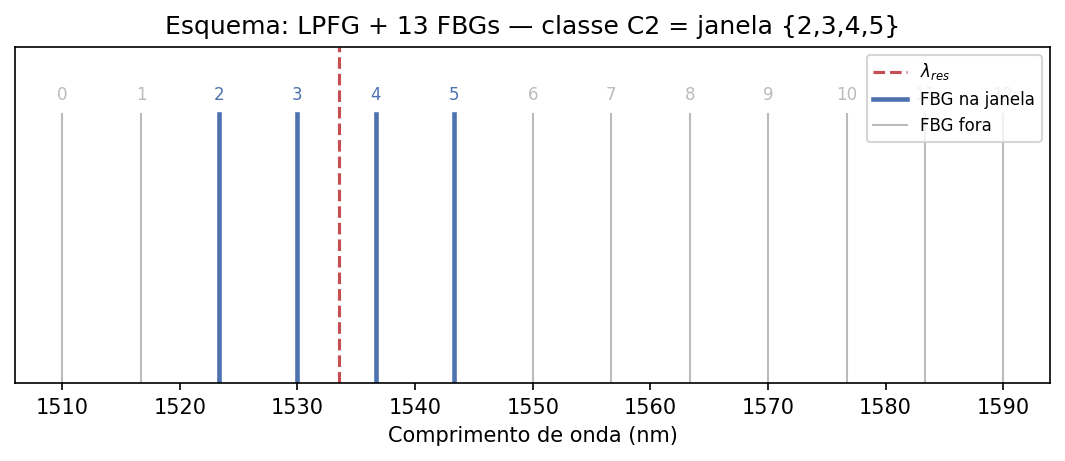
\includegraphics[width=\columnwidth]{fig_schema_lpg_fbg.png}
\caption{Esquema: LPFG (Lorentziana ilustrativa), $\lambda_{res}$ e janela-classe $C_s$ no array de 13 FBGs.}
\label{fig:schema}
\end{figure}

\section{Metodologia}

\subsection{Dados e pré-processamento}
Usamos o conjunto medido associado a~\cite{Barino2025TIM}.
No arranjo experimental de referência, LPFG e array de $13$ FBGs (centros aproximados entre $1510$ e $1590$~nm) são cascateados e lidos por um interrogador comercial de FBGs; a LPFG modula o perfil de refletividade visto pelo interrogador~\cite{Barino2025TIM}.
Há $8200$ amostras no arquivo bruto; o filtro $1515<\lambda_{res}<1585$~nm --- interior ao span do array --- produz $7300$ exemplos utilizáveis.
As potências são normalizadas por amostra (subtração do mínimo e divisão pela soma), como em~\cite{Barino2025TIM}, garantindo invariância a offset e escala global.
A Fig.~\ref{fig:heatmap} exibe $73$ amostras espalhadas ao longo do intervalo de $\lambda_{res}$: a faixa de alta potência desloca-se pelas colunas do array, embora $\lambda_{res}$ não apareça na figura.

A Tabela~\ref{tab:balance} quantifica o desbalanceamento.
$C_2$ concentra quase $29\%$ dos exemplos, enquanto $C_3$ e $C_9$ ficam abaixo de $1{,}5\%$.
Esse perfil explica por que F1 macro tende a ficar abaixo de F1 weighted e por que o AdaBoost necessitou de árvores mais profundas e pesos de classe.

\begin{table}[!t]
\caption{Distribuição das $10$ classes no conjunto filtrado ($N=7300$).}
\label{tab:balance}
\centering
\setlength{\tabcolsep}{3.5pt}
\begin{tabular}{lrr|lrr}
\toprule
Classe & $n$ & $\%$ & Classe & $n$ & $\%$ \\
\midrule
$C_0$ & 520 & 7{,}12 & $C_5$ & 542 & 7{,}42 \\
$C_1$ & 1257 & 17{,}22 & $C_6$ & 236 & 3{,}23 \\
$C_2$ & 2089 & 28{,}62 & $C_7$ & 696 & 9{,}53 \\
$C_3$ & 89 & 1{,}22 & $C_8$ & 270 & 3{,}70 \\
$C_4$ & 1501 & 20{,}56 & $C_9$ & 100 & 1{,}37 \\
\bottomrule
\end{tabular}
\end{table}

\begin{figure*}[!t]
\centering

\includegraphics[width=0.55\textwidth]{fig_fbg_power_heatmap_73x13.png}
\caption{Potências FBG normalizadas ($73$ de $7300$ amostras). A diagonal clara indica o deslocamento do padrão pelo array; $\lambda_{res}$ não é exibido.}
\label{fig:heatmap}
\end{figure*}

\subsection{Classificadores e hiperparâmetros}
Comparamos kNN, SVM~RBF, MLP, Random Forest, AdaBoost e MQ.
kNN, SVM, MLP e MQ usam \texttt{StandardScaler} ajustado apenas no treino de cada partição.
As grades de busca incluem, entre outros: $k\in\{3,5,7,11\}$ e pesos uniforme/distância (kNN); $C\in\{0{,}1,1,10\}$ e $\gamma\in\{\mathrm{scale},0{,}1\}$ (SVM); arquiteturas e regularização $\alpha$ (MLP); profundidade e número de árvores (RF); e, no AdaBoost, profundidade da árvore base $\in\{2,3,4\}$, $n_{\mathrm{estimators}}\in\{100,200\}$ e taxa de aprendizado $\in\{0{,}3,0{,}5,1{,}0\}$, sempre com \texttt{class\_weight=balanced}.
O consenso do AdaBoost no desenvolvimento foi profundidade~$4$, $200$ estimadores e taxa~$0{,}3$.

\subsection{Protocolo de avaliação}
Reservamos $20\%$ como hold-out estratificado por classe ($1460$ amostras), intacto até o teste final.
No desenvolvimento ($5840$), usamos \texttt{StratifiedKFold} com $5$ folds.
A estratificação por $y$ evita folds sem representantes de classes raras, o que seria especialmente problemático para $C_3$ e $C_9$.
Hiperparâmetros foram escolhidos por nested CV (\texttt{GridSearchCV} interno, $3$ folds, scorer $=$ acurácia), reduzindo viés otimista de ajustar e avaliar na mesma partição~\cite{Hastie2009ESL}.
Os modelos de consenso foram retreinados no desenvolvimento completo e avaliados uma única vez no hold-out.
Reportamos acurácia e F1 weighted na tabela principal; F1 macro e matrizes de confusão sustentam a discussão de classes raras.
Implementações seguem a biblioteca \texttt{scikit-learn}, com semente fixa para reprodutibilidade.

\section{Resultados}

\subsection{Desempenho agregado}
A Tabela~\ref{tab:results} coloca CV e hold-out na mesma visão.
SVM lidera a CV ($0{,}934\pm0{,}004$) e empata com Random Forest no hold-out ($0{,}938$).
AdaBoost, após o ajuste descrito, entra no pelotão intermediário-alto ($0{,}923$ no hold-out), bem acima do baseline linear MQ ($0{,}789$), indicando que a fronteira potências$\to$janela é essencialmente não linear.
O gap entre F1 weighted e F1 macro (omitido da tabela por espaço, porém observado em todos os métodos) acompanha o desbalanceamento da Tabela~\ref{tab:balance}.

\begin{table}[!t]
\caption{Desempenho multiclasse: CV (média $\pm$ desvio) e hold-out (HO).}
\label{tab:results}
\centering
\setlength{\tabcolsep}{2.6pt}
\begin{tabular}{lcccc}
\toprule
Método & Acc.\ CV & F1$_w$ CV & Acc.\ HO & F1$_w$ HO \\
\midrule
SVM & $\mathbf{0{,}934\pm0{,}004}$ & $0{,}927$ & $\mathbf{0{,}938}$ & $0{,}931$ \\
RF & $0{,}929\pm0{,}004$ & $0{,}923$ & $\mathbf{0{,}938}$ & $0{,}932$ \\
AdaBoost & $0{,}924\pm0{,}004$ & $0{,}923$ & $0{,}923$ & $0{,}925$ \\
MLP & $0{,}919\pm0{,}011$ & $0{,}908$ & $0{,}933$ & $0{,}923$ \\
kNN & $0{,}907\pm0{,}003$ & $0{,}901$ & $0{,}919$ & $0{,}911$ \\
MQ & $0{,}779\pm0{,}007$ & $0{,}736$ & $0{,}789$ & $0{,}750$ \\
\bottomrule
\end{tabular}
\end{table}

\subsection{Erros versus $\lambda_{res}$}
A Fig.~\ref{fig:lambda} mostra a acurácia do SVM por faixas de $\lambda_{res}$ (predições da CV empilhadas).
Faixas centrais do intervalo útil são tipicamente mais fáceis; a degradação concentra-se em ${\approx}1548$--$1580$~nm, região em que classes de janela periféricas e amostras mais escassas se combinam.
Essa visão é complementar à Tabela~\ref{tab:results}: o mesmo modelo ``médio'' esconde heterogeneidade espectral.

\begin{figure}[!t]
\centering
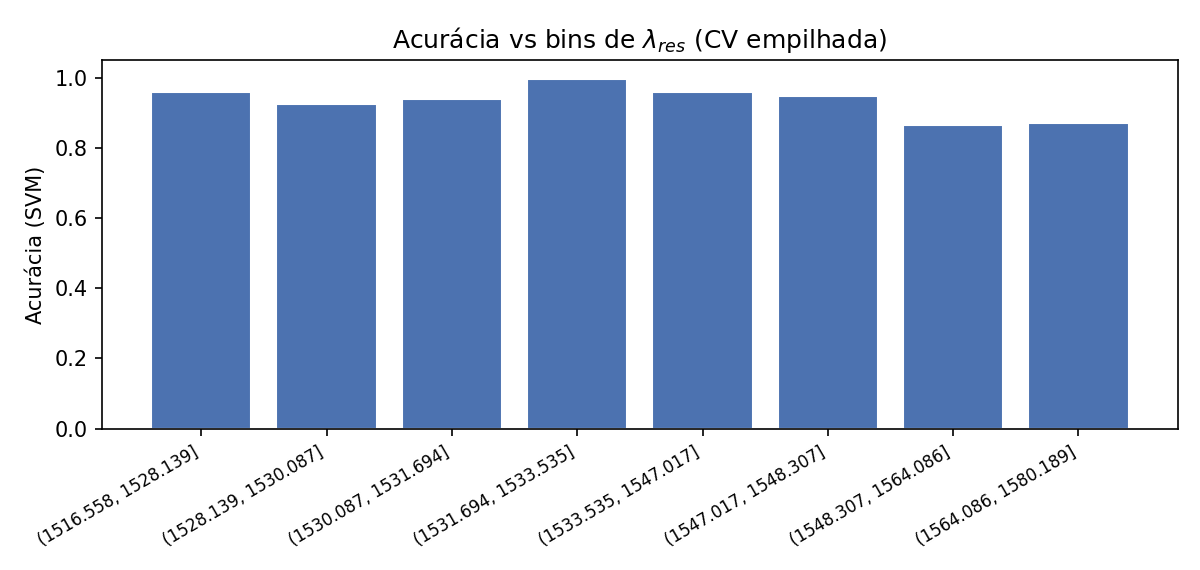
\includegraphics[width=\columnwidth]{fig_acc_vs_lambda.png}
\caption{Acurácia do SVM por bin de $\lambda_{res}$ (CV empilhada).}
\label{fig:lambda}
\end{figure}

\subsection{Matriz de confusão}
A Fig.~\ref{fig:cm} compara as matrizes do SVM e do Random Forest no hold-out, normalizadas por linha.
Os erros residuais ocorrem sobretudo entre classes adjacentes --- coerente com a sobreposição de três FBGs entre $C_s$ e $C_{s+1}$.
Do ponto de vista da cascata classificação$\to$regressão, confundir janelas vizinhas é menos grave do que saltos longos no array, pois o subconjunto de canais permanece parcialmente correto.
O padrão qualitativo semelhante nos dois melhores métodos reforça que o empate em acurácia não é coincidência isolada: ambos capturam a geometria das janelas no espaço de potências.
Diferenças pontuais em classes raras são esperadas dada a baixa contagem absoluta (Tabela~\ref{tab:balance}).

\begin{figure*}[!t]
\centering
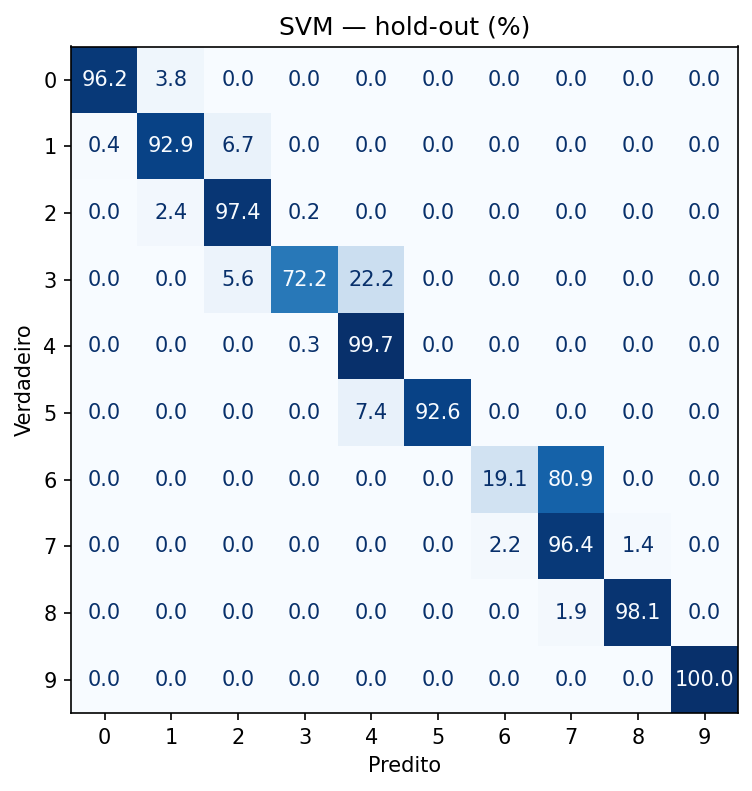
\includegraphics[width=0.45\textwidth]{cm_agg_SVM_pct.png}\hfill

\includegraphics[width=0.45\textwidth]{cm_agg_RandomForest_pct.png}
\caption{Matrizes de confusão no hold-out (\% por linha): esquerda, SVM; direita, Random Forest.}
\label{fig:cm}
\end{figure*}

\subsection{Ablação: posições Bragg}
Concatenar $\boldsymbol{\lambda}_{\mathrm{FBG}}$ às potências altera o ranking de forma desigual: MLP ($+0{,}029$ em acurácia CV), Random Forest ($+0{,}019$) e MQ ($+0{,}041$) melhoram; o SVM permanece quase neutro; o kNN piora ($-0{,}050$).
A Fig.~\ref{fig:feat} resume essa comparação lado a lado.
Interpretamos o prejuízo do kNN como sensibilidade à mudança de escala/dimensionalidade sob distância euclidiana.
Para o MQ, as posições adicionam informação linearmente útil que as potências sozinhas não carregam de modo suficiente; para o SVM RBF, as potências já induzem uma margem competitiva sem as coordenadas Bragg.

\begin{figure}[!t]
\centering

\includegraphics[width=\columnwidth]{passo5_compare_features.png}
\caption{Acurácia CV: somente potências versus potências concatenadas às posições Bragg.}
\label{fig:feat}
\end{figure}

\section{Discussão}

Formalizar a seleção de FBGs como dez classes alinha o problema à avaliação clássica de reconhecimento de padrões e torna explícito o conjunto de decisões~\cite{Hastie2009ESL}.
Em relação à regressão de~\cite{Barino2025TIM}, o classificador atua como estágio anterior: se $C_s$ for predito corretamente, um estimador de $\lambda_{res}$ pode operar apenas sobre quatro canais, potencialmente reduzindo ruído de FBGs irrelevantes --- hipótese ainda não medida em RMSE.

Do ponto de vista de engenharia de sensores, a cascata classificação$\to$regressão também facilita diagnóstico: falhas de demodulação podem ser atribuídas à janela errada (Fig.~\ref{fig:cm}) ou à estimação contínua dentro da janela correta.
Além disso, um classificador raso (SVM/RF) é barato de retreinar quando o array FBG é recalibrado, enquanto o modelo de autoatenção de~\cite{Barino2025TIM} permanece responsável pela precisão submetrica de $\lambda_{res}$.

O desempenho de SVM/RF ($0{,}938$ no hold-out) indica que a etapa de janela é tratável com modelos clássicos.
Por outro lado, o desbalanceamento (Tabela~\ref{tab:balance}) e a otimização por acurácia favorecem classes majoritárias: estratégias futuras incluem scorer macro-F1, reamostragem ou custos assimétricos, sobretudo para $C_3$ e $C_9$.
Confusões adjacentes, embora preferíveis a erros longos, ainda podem deslocar a estimação de $\lambda_{res}$ em frações de nanômetro se a regressão for sensível ao canal excluído/incluído indevidamente.

Limitações: (i)~não quantificamos o ganho de RMSE ao fixar a janela antes da regressão; (ii)~o protocolo usa um único hold-out (além da CV), suficiente para o escopo da disciplina, porém sensível à partição; (iii)~não exploramos modelos profundos na classificação, propositalmente, para isolar o ganho da formulação multiclasse; (iv)~a Lorentziana da Fig.~\ref{fig:schema} é ilustrativa, não um espectro medido.

\section{Conclusão}

Formulamos a seleção das FBGs relevantes à demodulação de LPFG como classificação multiclasse com dez janelas contíguas $C_s$, explorando a contiguidade observada nos dados filtrados.
Com potências normalizadas de um array de $13$ FBGs, nested CV e hold-out estratificado, SVM e Random Forest alcançaram acurácia $0{,}938$ no teste final; erros remanescentes concentram-se em classes adjacentes e em faixas de $\lambda_{res}$ menos povoadas.
A ablação com posições Bragg mostra ganhos dependentes do indutor, reforçando que a representação deve ser escolhida junto com o classificador.
O trabalho estabelece a Parte~1 de uma arquitetura em cascata cuja Parte~2 --- estimação de $\lambda_{res}$ restrita à janela predita, na linha de~\cite{Barino2025TIM} --- permanece como próximo passo experimental.

\FloatBarrier
\bibliographystyle{IEEEtran}
\bibliography{references}

\end{document}
